\documentclass[10pt,twocolumn,letterpaper]{article}

\usepackage{cvpr}
\usepackage{times}
\usepackage{epsfig}
\usepackage{graphicx}
\usepackage{subfig}
\usepackage{amsmath}
\usepackage{bm}
\usepackage{amssymb}

% Include other packages here, before hyperref.

\graphicspath{{../assets/}}
% If you comment hyperref and then uncomment it, you should delete
% egpaper.aux before re-running latex.  (Or just hit 'q' on the first latex
% run, let it finish, and you should be clear).
\usepackage[breaklinks=true,bookmarks=false]{hyperref}

\cvprfinalcopy % *** Uncomment this line for the final submission

\def\httilde{\mbox{\tt\raisebox{-.5ex}{\symbol{126}}}}

% Pages are numbered in submission mode, and unnumbered in camera-ready
%\ifcvprfinal\pagestyle{empty}\fi
\setcounter{page}{1}
\begin{document}

%%%%%%%%% TITLE
\title{Content-Aware Image Resizing with Seam Carving and ResNets}

\author{Shane Segal\\
  York University\\
  Toronto ON, Canada\\
  {\tt\small smsegal@eecs.yorku.ca}
}

\maketitle
%\thispagestyle{empty}

%%%%%%%%% ABSTRACT
\begin{abstract}
  Image resizing that respects the semantic content of images is an improvement
  on prior methods of Content Aware Image resizing that don't integrate
  higher-level knowledge of the image into their resizing processes. We present
  an algorithm that combines the capabilities of modern, state of the art deep
  learning techniques with the classical Seam Carving algorithm
  \cite{seamcarve}. By combining the ability of \cite{seamcarve} and the
  advanced image segmentation techniques of Mask~{R-CNN} \cite{maskrcnnpaper},
  semantically irrelevant information is removed from the image, while regions
  featuring subjectively important content is retained. In addition, the image
  enlarging capabilities of the original seam carving algorithm are enhanced by
  avoiding distortions of higher level features when they are present in the
  image.
\end{abstract}

%%%%%%%%% BODY TEXT
\section{Introduction}

Image resizing has historically been done by cropping or scaling images, to
shrink or enlarge them respectively. The introduction of the seam-carving
operator by \cite{seamcarve} allowed for the easy resizing of images while
preserving spots of the image according to some energy function. The original
paper used the gradient magnitude of the image as the energy function in order
to eliminate areas of low change, which is a reasonable proxy for
``uninteresting'' parts of an image.

Content-Aware image resizing, also referred to as image retargetting, is an
interesting problem as it provides quick and immediate feedback regarding the
success of an approach. In addition, it is one application of a larger problem
of exploring what kinds of content and patterns are visually arresting to the
human visual system. The heuristic to determine human interest in the original
paper is both simple and effective for many classes of image.

Seam Carving works quite well when applied to landscapes or other images where
there are large patches of low and high variation. However, when applied to
images with features that people are particularly attentive to (such as faces)
the results can be noticeably bad and distorted. See Figure
\ref{fig:laughcomparison} for a comparison between our method and the original seam
carving algorithm (reimplemented for this paper).

By combining the ability to selectively remove ``uninteresting'' parts of the
image with the ability to detect high level features at an accuracy that can't
be matched by a gradient based approach, we demonstrate adaptive image resizing
that preserves faces and other high level content in a subjectively more
pleasing and natural way.

\begin{figure}[t]
  \centering
  \subfloat[Original]{{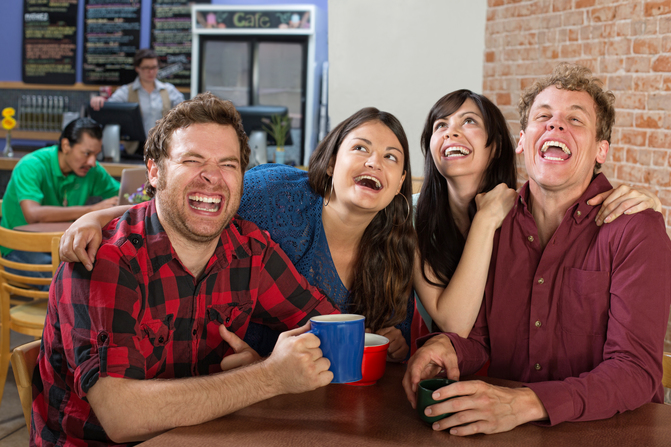
\includegraphics[width=0.8\linewidth]{people-laughing}}}
  \qquad
  \subfloat[Seam-Carving]{{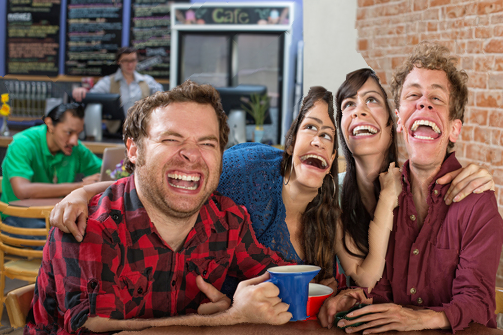
\includegraphics[width=0.8\linewidth]{badlaughcarve}}}
  \qquad
  \subfloat[Our Method]{{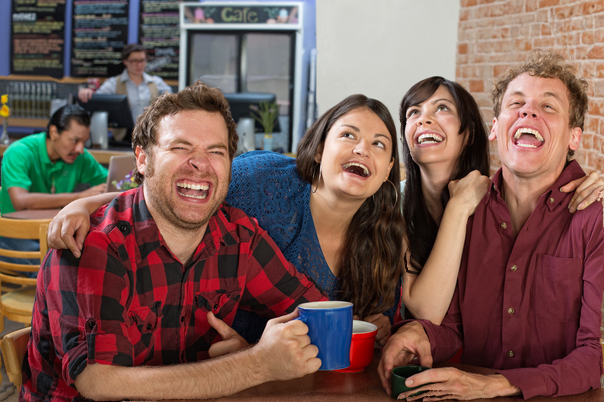
\includegraphics[width=0.8\linewidth]{smallfancylaughbest}}}
  \caption{Comparison between the original method and our own. The bottom two
    images are 80\% of the size of the original image.}
  \label{fig:laughcomparison}
\end{figure}

%-------------------------------------------------------------------------
\section{Prior Work}

Seam Carving \cite{seamcarve} works by selecting seams of the lowest energy in
an image, and continuously removing them until a target size is reached. A seam
is a connected path leading from one end to the other of an image in a
particular dimension. Let $\boldsymbol{I}$ be an $n \times m$ image. Using the notation of
the original paper, a vertical seam is:

\begin{equation}
  \boldsymbol{s^x} = \{s_i^x\}_{i=1}^n = \{(x(i),i)\}_{i=1}^n, \text{s.t } \forall{i}, |x(i) - x(i-1)| \leq 1
\end{equation}

where $x$ is a mapping of: $[1,...,n] \rightarrow [1,...,m]$. This is a
connected path of pixels running from top to bottom of the image, with exactly
one mapping between a row $x(i)$ and the horizontal location of the seam at that
row. In the same way, a horizontal path consists of a mapping $y: [1,...,m]
\rightarrow [1,...,n]$, and:

\begin{equation}
  \boldsymbol{s^y} = \{s_j^y\}_{j=1}^n = \{(y(j),j)\}_{j=1}^n, \text{s.t } \forall{j}, |y(j) - y(j-1)| \leq 1
\end{equation}

The pixels of the seam are therefore:
\begin{equation}
  \boldsymbol{I}_s = \{\boldsymbol{I}(s_i)\}_{i=1}^n = \{\boldsymbol{I}(x(i),i)\}_{i=1}^n
\end{equation}

Since seams are always of $1 \times n$ or $m \times 1$, their removal from an
image will cause a reduction of exactly one pixel in either the width or height
of the target image.

With this idea, the optimal seam to remove from an image will be the one that
minimizes the cost, where the cost is defined as the sum of the energy of the
seam, where the energy can be an arbitrary function. The optimal seam $s^*$ is
the one that minimizes this energy over the range of possible seams for a given
dimension of the image:
\begin{equation}
  s^* = \min_s(E(s)) = \min_s \sum_{i=1}^n{e(\boldsymbol{I}(s_i))}
\end{equation}

The optimal seam can be found through a bottom-up dynamic programming approach,
where we can create a scoring matrix $M$ by computing the minimum energy for all
possible connected seams at a point by:

\begin{equation*}
  M(i, j) = e(i, j) + \min(M(i - 1, j - 1),M(i - 1, j),M(i - 1, j+1))
\end{equation}

After the scoring matrix is constructed, we can find the optimal seam by tracing
up from the bottom and picking the minimum value of the three connected elements
on the row above. The process is identical for horizontal seams, using the
transpose of the original image.

After the seam is found, it can be removed from the image and the whole process
can be repeated until the desired image size in the specified dimension
$n' \leq n$ is reached. A simplification from the original paper is made here.
The authors propose a scheme for finding the optimal removal order of seams, but
the qualitative difference in the modified image was negligible. A simpler
approach was taken by simply applying horizontal seam removal to an image, and
then transposing the resulting image and performing the process again, until the
desired size was reached in each dimension.

To enlarge an image from $n \times m$ to $n' \times m'$, it is not sufficient to
simply add the optimal seam repeatedly, as this will most often insert the same
seam repeatedly, causing obvious banding effects as seen in Figure
\ref{fig:seaminsertion}.

\begin{figure}[t]
  \begin{center}
    \subfloat[Optimal Seam Insertion]{{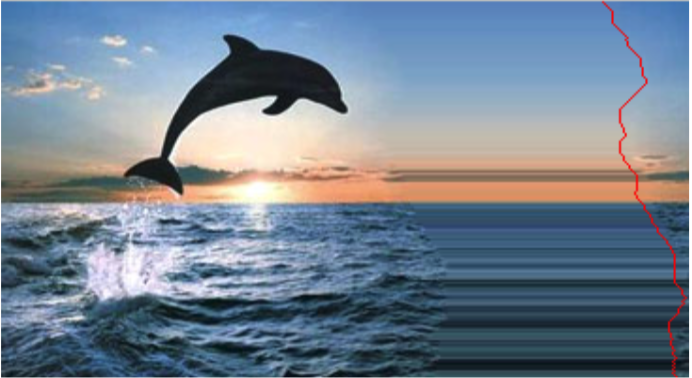
\includegraphics[width=0.8\linewidth]{badseaminsertion}}}
    \qquad
    \subfloat[Seams Inserted in order of Removal]{{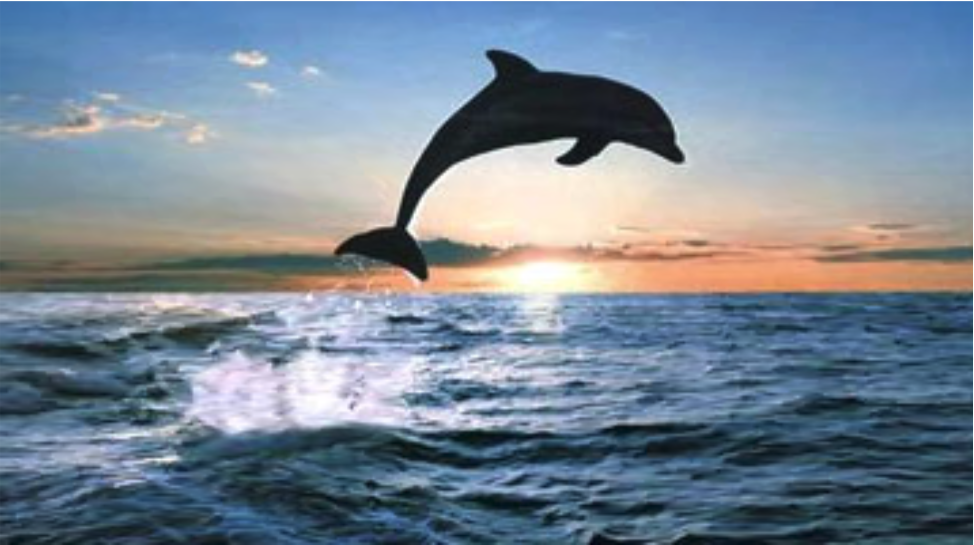
\includegraphics[width=0.8\linewidth]{goodseaminsertion}}}
    \caption{The result of inserting the optimal seam repeatedly and in order of
      removal. (Figures taken from \cite{seamcarve})}
    \label{fig:seaminsertion}
  \end{center}
\end{figure}

To avoid this issue, it suffices to first shrink the image by $(n' - n, m' - m)$
and then save the seams in the order of removal. After the image is fully
resized, you then insert the removed seams back into the original image.

The energy function is generally the gradient magnitude of the image,
as the original authors experimented with different functions but all provided
qualitatively similar results.

\subsection{Limitations of Prior Work}

The Seam Carving method described above works very well for images with clearly
seperated regions of high and low energy, and especially those without faces or
other features that human minds are particularly sensitive towards. An example
of a good image to perform seam carving on is seen in Figure
\ref{fig:goodcarve}.

\begin{figure}[t]
  \centering
  \subfloat[Original Image]{{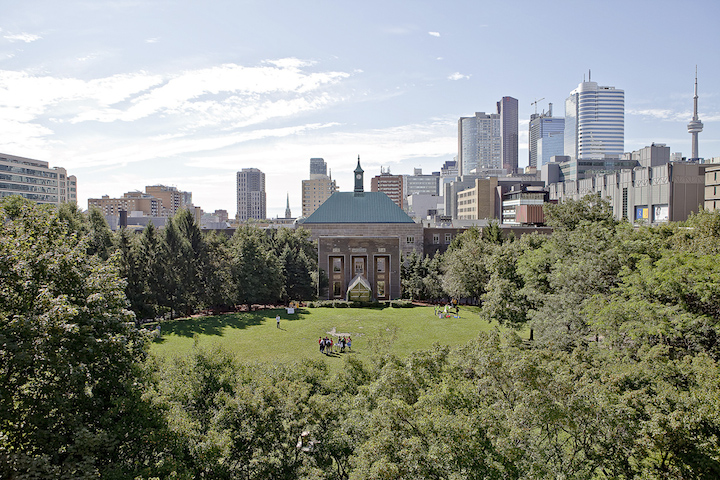
\includegraphics[width=0.8\linewidth]{ryerson}}}
  \qquad
  \subfloat[Shrunk by 20\%]{{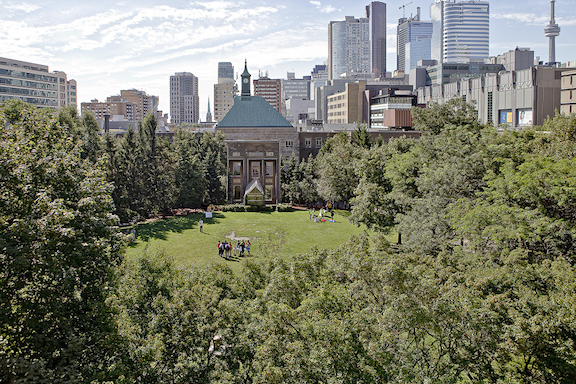
\includegraphics[width=0.8\linewidth]{ryesmall}}}
  \qquad
  \subfloat[Grown by 20\%]{{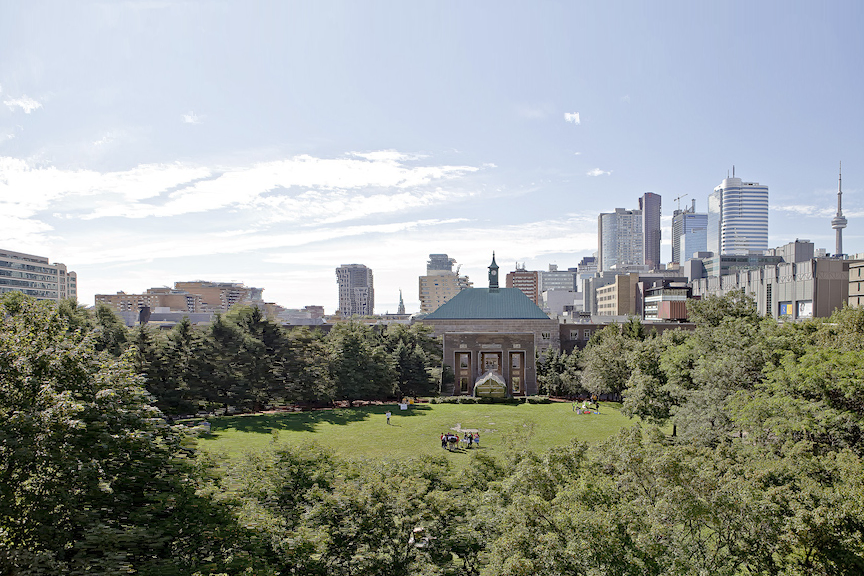
\includegraphics[width=0.8\linewidth]{ryelarge}}}
  \caption{An image with good results shown with classical seam carving.}
  \label{fig:goodcarve}
\end{figure}

However, when seam carving is applied to images with faces or other high level
semantic features, the results are often wildly distorted. This is because the
idea of gradient magnitude being a perfect measure of human attention in an
image is innacurate at best. An example of this can be seen in Figure
\ref{fig:badcarving}.

\begin{figure}
  \centering
  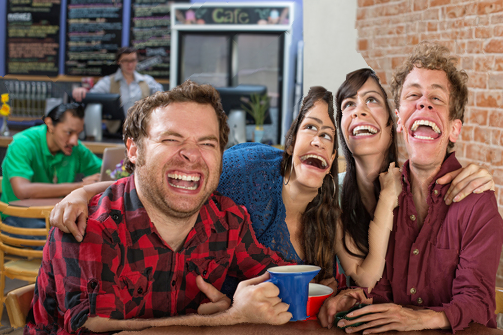
\includegraphics[width=0.8\linewidth]{badlaughcarve}
  \caption{Seam Carving gone wrong.}
  \label{fig:badcarving}
\end{figure}

Other limitations include only being able to enlarge an image by a factor of 2
as seams have to be removed first before they can be added back to the original.

\subsection{Addressing the Limitations}
This paper seeks to address the inability to resize images containing human
images and other recognizable object categories. By utilizing the neural network
defined in \cite{maskrcnnpaper, matterport_maskrcnn_2017}, the high level
feature knowledge embedded in the pretrained network weights allow our algorithm
to preserve the semantic content of the images being resized. This not only
allows for better shrinking of images, it also allows for better enlarging by
the same strategy. We enhance the energy function by introducing the masks
generated by Mask R-CNN as a measure of greater importance to the areas
belonging to high level features.

%-------------------------------------------------------------------------
\section{Datasets}
A selection of images have been taken from Flickr, which contain a Creative
Commons fair use license. These images have been selected for evaluation as they
present the kinds of features the original seam carving algorithm did not
perform well on.

\section{System Description}
The seam carving system described in the original paper was entirely
reimplemented in the Julia programming language. This language was chosen for
its greater ease of use and speed over Matlab, and chosen over Python for it's
increased speed. The metaprogramming and extensive linear algebra and image
filtering/manipulation features of Julia made several aspects of the
reimplementation easier and faster than an equivalent Matlab or Python
implementation. The only high level image filtering features of Julia used was
the image gradient calculation. Otherwise, the seam-carving portion of the
algorithm has been entirely implemented based on \cite{seamcarve}. The Mask-RCNN
implementation used is written in Python with TensorFlow, and is communicating
with Julia through an interface library called PyCall. 

Mask-RCNN is used to calculate the mask overlays of the high level objects in
the image. As there is a separate overlay for each specific mask, these are
summed and normalized into a single image with pixels inside the mask being $\alpha$
and those outside being 1. The mask sum is computed by:

\begin{equation}
  \boldsymbol{R} = \alpha \sum_{i=1}^N{R_i}+ \boldsymbol{1}
\end{equation}

where $\boldsymbol{1}$ is a matrix of ones the same size as $R_i$, and $\alpha$
is a hyperparameter chosen experimentally to improve the preservation of
semantic content in the image. Unless otherwise stated, $\alpha = 20$ for images
using our algorithm.

We then element-wise multiply (sometimes known as the ``Hadamard Product''
denoted by $\oplus$) our gradient magnitude by $\boldsymbol{R}$ to produce our
energy matrix:

\begin{equation}
  E(\boldsymbol{I}) = |\frac{\delta \boldsymbol{I}}{\delta x}^2 + \frac{\delta \boldsymbol{I}}{\delta y}^2| \oplus \boldsymbol{R}
\end{equation}

After our modified energy matrix is produced, the classical seam-carving
algorithm is followed.

\subsection{Running Time}

When run without the inclusion of Mask-RCNN, our seam carving implementation
runs quite fast, in 

\begin{equation}
  \boldsymbol{O}\left((n'-n)(m'-m) + \sum_{i=n}^{n'}{i} + \sum_{j=m}^{m'}{j} \right) = \boldsymbol{O}(NM)
\end{equation}

time, where the sums are the cost of computing a seam at each image size, and
$(N, M) = (n' - n, m' - m)$ meaning it is linear in the number of seams to
remove.

When scaling an $(432,768)px$ image from $[0.5,...,1.5]$ in increments of $0.1$,
we see that the execution times are what we expect, following a generally
parabolic distribution, as $M, N$ are changing at the same rate. In addition, we
can expect a constant factor to be added to the execution time of growth images,
as they must first remove, and then add back the seams to the image. See Figure
\ref{fig:execplotnornn}.

The addition of the RNN to the algorithm contributes greatly to both the
subjective quality of the results, and unfortunately the execution time.
However, this appears to be a constant factor and not a time complexity
increase. As can be seen in Figure \ref{fig:execplotrnn}, when plotted from
a scale of $[0.8,...,1.2]$ on the same image, we see that the execution time is much larger.

\begin{figure}
  \centering
  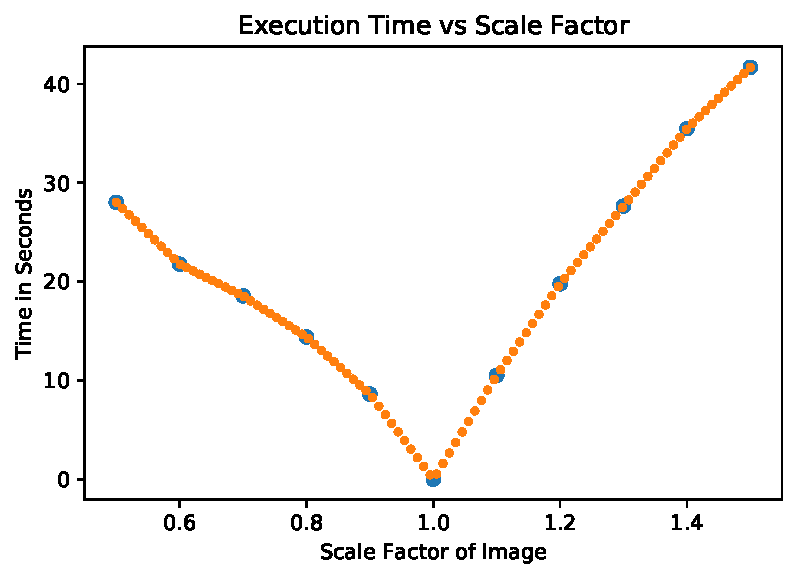
\includegraphics[width=0.9\linewidth]{nornntimes}
  \caption{Execution Time Vs Scale Factor for basic Seam Carving}
  \label{fig:execplotnornn}
\end{figure}

\begin{figure}
  \centering
  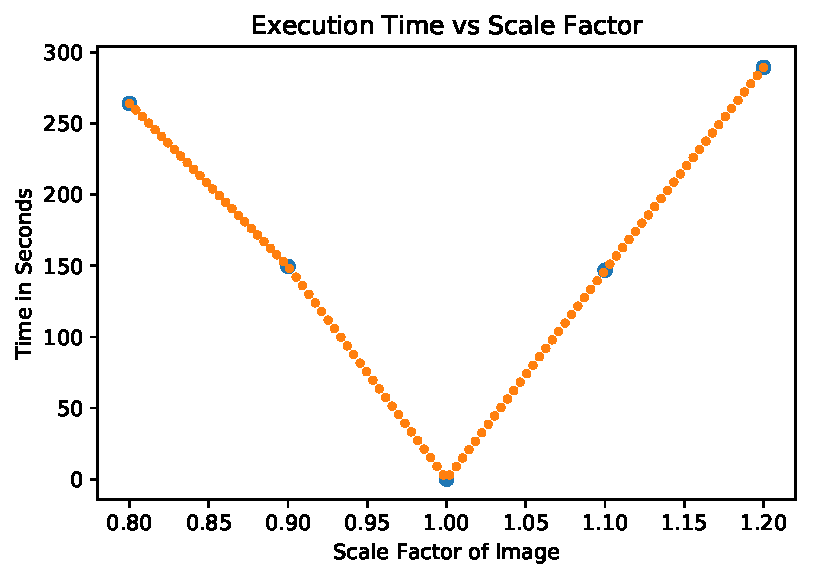
\includegraphics[width=0.9\linewidth]{rnntimes}
  \caption{Execution Time Vs Scale Factor for Mask-RNN and Seam Carving}
  \label{fig:execplotrnn}
\end{figure}


\begin{table}[htbp]
  \centering
  \begin{tabular}{rr}
    Scale & Execution Time (seconds)\\
    \hline
    0.5 & 28.008397\\
    0.6 & 21.751526\\
    0.7 & 18.539442\\
    0.8 & 14.389925\\
    0.9 & 8.604313\\
    1.0 & 0.002406\\
    1.1 & 10.512507\\
    1.2 & 19.771803\\
    1.3 & 27.629700\\
    1.4 & 35.464424\\
    1.5 & 41.666718\\
  \end{tabular}
  \caption{Execution time and scale factors for resizing an image without RNN}
  \label{table:exectimenornn}
\end{table}

\section{Conclusion}
\subsection{What Have We Discovered?}
One of the main discoveries of this project was the ability of simple methods to
provide complex and interesting results. It is common today to assume that
Deep Learning and other Machine Learning methods are required to get good
results, but the results of the plain seam carving algorithm are impressive even
when held against more modern methods.

However, that is not to say that Deep Learning and associated methods do not
have their place. In fact, our combination of classical methods and Deep methods
highlights an important synergy that can drive good results in research going
forwards.

\subsection{Future Work}
In the future, the main aspect to be improved is the execution time of the
improved content aware image resizing algorithm. A possible way to do this is to
eliminate the overhead of having to recompute the masks on each iteration. A
possible way to do this is to compute the initial masks, and then combine it
with the gradient space of the image, and perform seam-carving in the gradient
space entirely, reconstruction the final image using Poisson Reconstruction
\cite{poisson}, as was mentioned in \cite{seamcarve}. This should offer
tremendous speed up, as we would avoid having to recompute the image masks, as
well as eliminate most of the overhead of calling a Python Library from within
Julia.

Additional testing can also be done with higher values of $\alpha$. When testing
values much beyond 20, there seems to be some kind of instability in the
library, causing crashes more often than desired during execution. This is
especially unfortunate considering the length of the execution time needed for
the integrated RNN-Seam Carving algorithm.

There are additional optimizations that can be made to the original
seam-carving application that can greatly increase the speed of its execution
such as implementing a neighbour-based approach to calculating seams that was
capable of real-time computation back in 2009 \cite{fastcarve}. However, as
there is no discrete phase of energy computation, it is unclear how to adapt our
system to this faster method.
%------------------------------------------------------------------------
\section{Additional Images}

All text must be in a two-column format. The total allowable width of the
text area is $6\frac78$ inches (17.5 cm) wide by $8\frac78$ inches (22.54
cm) high. Columns are to be $3\frac14$ inches (8.25 cm) wide, with a
$\frac{5}{16}$ inch (0.8 cm) space between them. The main title (on the
first page) should begin 1.0 inch (2.54 cm) from the top edge of the
page. The second and following pages should begin 1.0 inch (2.54 cm) from
the top edge. On all pages, the bottom margin should be 1-1/8 inches (2.86
cm) from the bottom edge of the page for $8.5 \times 11$-inch paper; for A4
paper, approximately 1-5/8 inches (4.13 cm) from the bottom edge of the
page.

%-------------------------------------------------------------------------
\subsection{Margins and page numbering}

All printed material, including text, illustrations, and charts, must be kept
within a print area 6-7/8 inches (17.5 cm) wide by 8-7/8 inches (22.54 cm)
high.
Page numbers should be in footer with page numbers, centered and .75
inches from the bottom of the page and make it start at the correct page
number rather than the 4321 in the example.  To do this fine the line (around
line 23)
\begin{verbatim}
%\ifcvprfinal\pagestyle{empty}\fi
\setcounter{page}{4321}
\end{verbatim}
where the number 4321 is your assigned starting page.

Make sure the first page is numbered by commenting out the first page being
empty on line 46
\begin{verbatim}
%\thispagestyle{empty}
\end{verbatim}


%-------------------------------------------------------------------------
\subsection{Type-style and fonts}

Wherever Times is specified, Times Roman may also be used. If neither is
available on your word processor, please use the font closest in
appearance to Times to which you have access.

MAIN TITLE. Center the title 1-3/8 inches (3.49 cm) from the top edge of
the first page. The title should be in Times 14-point, boldface type.
Capitalize the first letter of nouns, pronouns, verbs, adjectives, and
adverbs; do not capitalize articles, coordinate conjunctions, or
prepositions (unless the title begins with such a word). Leave two blank
lines after the title.

AUTHOR NAME(s) and AFFILIATION(s) are to be centered beneath the title
and printed in Times 12-point, non-boldface type. This information is to
be followed by two blank lines.

The ABSTRACT and MAIN TEXT are to be in a two-column format.

MAIN TEXT. Type main text in 10-point Times, single-spaced. Do NOT use
double-spacing. All paragraphs should be indented 1 pica (approx. 1/6
inch or 0.422 cm). Make sure your text is fully justified---that is,
flush left and flush right. Please do not place any additional blank
lines between paragraphs.

Figure and table captions should be 9-point Roman type as in
Figures~\ref{fig:onecol} and~\ref{fig:short}.  Short captions should be centred.

\noindent Callouts should be 9-point Helvetica, non-boldface type.
Initially capitalize only the first word of section titles and first-,
second-, and third-order headings.

FIRST-ORDER HEADINGS. (For example, {\large \bf 1. Introduction})
should be Times 12-point boldface, initially capitalized, flush left,
with one blank line before, and one blank line after.

SECOND-ORDER HEADINGS. (For example, { \bf 1.1. Database elements})
should be Times 11-point boldface, initially capitalized, flush left,
with one blank line before, and one after. If you require a third-order
heading (we discourage it), use 10-point Times, boldface, initially
capitalized, flush left, preceded by one blank line, followed by a period
and your text on the same line.

%-------------------------------------------------------------------------
\subsection{Footnotes}

Please use footnotes\footnote {This is what a footnote looks like.  It
often distracts the reader from the main flow of the argument.} sparingly.
Indeed, try to avoid footnotes altogether and include necessary peripheral
observations in
the text (within parentheses, if you prefer, as in this sentence).  If you
wish to use a footnote, place it at the bottom of the column on the page on
which it is referenced. Use Times 8-point type, single-spaced.


%-------------------------------------------------------------------------
\subsection{References}

List and number all bibliographical references in 9-point Times,
single-spaced, at the end of your paper. When referenced in the text,
enclose the citation number in square brackets, for
example~\cite{Authors14}.  Where appropriate, include the name(s) of
editors of referenced books.

\begin{table}
\begin{center}
\begin{tabular}{|l|c|}
\hline
Method & Frobnability \\
\hline\hline
Theirs & Frumpy \\
Yours & Frobbly \\
Ours & Makes one's heart Frob\\
\hline
\end{tabular}
\end{center}
\caption{Results.   Ours is better.}
\end{table}

%-------------------------------------------------------------------------
\subsection{Illustrations, graphs, and photographs}

All graphics should be centered.  Please ensure that any point you wish to
make is resolvable in a printed copy of the paper.  Resize fonts in figures
to match the font in the body text, and choose line widths which render
effectively in print.  Many readers (and reviewers), even of an electronic
copy, will choose to print your paper in order to read it.  You cannot
insist that they do otherwise, and therefore must not assume that they can
zoom in to see tiny details on a graphic.


%-------------------------------------------------------------------------
\subsection{Color}

Please refer to the author guidelines on the CVPR 2018 web page for a discussion
of the use of color in your document.

%------------------------------------------------------------------------
\section{Final copy}

You must include your signed IEEE copyright release form when you submit
your finished paper. We MUST have this form before your paper can be
published in the proceedings.

Please direct any questions to the production editor in charge of these
proceedings at the IEEE Computer Society Press: Phone (714) 821-8380, or
Fax (714) 761-1784.

{\small
\bibliographystyle{ieee}
\bibliography{egbib}
}

\end{document}
